%-------------------------------------------------
% CHAPTER 2
% This is a separate document for the Chapter 2, which is loaded into the main document.
%-------------------------------------------------

%% Chapter 02 will layout standard guidelines for font types and sizes 
%% The following are the available font sizes ranging from smallest to largest.



\section{Introduction}

This chapter gives some examples of how to change font sizes, families, styles and colors. Font size  commands change to size of the font. Font families change the typeface of the font. By default, LaTeX is set to the serif typeface (a.k.a. roman). Font styles refer to such things as bold, italics and underlined. Colours can be adjusted for the font, the font background and the page colour. 


\section{Font Sizes}

Font sizes are identified by special tags or commands, the actual size is not absolute but relative to the font size declared in the documentclass statement found at the start of the main.tex file.

\vspace{0.3cm}

\underline{This is a list of special tags for changing the font size}
\begin{verbatim}
\tiny 
\scriptsize
\footnotesize
\small
\normalsize
\large
\Large
\LARGE
\huge
\Huge
\end{verbatim}



If we use a set of curly brackets after the font tag, for example, \verb|\Large{text}| then only the text inside the brackets will be affected by the font tag command. In this sentence the {\huge huge font size} is set within the curly brackets \verb|{}| and then we can change to the {\footnotesize Foot note size font at the end of the sentence}. When we resume typing the font size will be back to normal because we set the huge font and footnote font inside the curly brackets. 

\vspace{0.3cm}

If we write the font tag without curly brackets, then the size that we set will become the default size from that point onward unless it is changed. For example, in the next sentence I will use the \verb|\footnotesize| font spacial tag. \footnotesize This font is written in footnotesize font without curly brackets. 

\vspace{0.4cm}

If I create a new paragraph the font size will still be set the footnotesize. In order to change the font size back we need to issue the \verb|\normalsize| font special tag. \normalsize This font is now set back to normal size.     

\vspace{0.4cm}

Next I will give examples of each of the font sizes. 

\vspace{0.4cm}


The following text is written in the {\tiny tiny font size.} 

The following text is written in the {\scriptsize scriptsize font size.} 

The following text is written in the {\footnotesize footnotesize font size.} 

The following text is written in the {\small small font size.} 

The following text is written in the {\normalsize normal font size.} 

The following text is written in the {\large large font size.} 

The following text is written in the {\Large Large font size.} Note the difference between large and Large with the use of the capital L for the larger version. 

The following text is written in the {\LARGE LARGE font size.} Note again the font size LARGE has all capital letters.

The following text is written in the {\huge huge font size.} 

The following text is written in the {\Huge Huge font size.} Again, note the difference between huge and Huge Large with the use of the capital H for the larger version. 

\newpage

\section{Font Families}

Font families change the typeface of the font. By default, LaTeX is set to the serif typeface (a.k.a. roman). There are other typefaces such as sans serif and typewriter.

{\fontfamily{qcr}\selectfont This text uses Gyre Cursor font typeface}

{\fontfamily{ptm}\selectfont This text uses the times font typeface}

{\fontfamily{put}\selectfont This text uses the utopia / fourier font typeface}

{\fontfamily{pcr}\selectfont This text uses the courier font typeface}

 {\fontfamily{cmss}\selectfont This text uses the Computer Modern Sans Serif font typeface}

\newpage

\section{Font Styles}

Font styles generally refer to such elements as bold, italics and underlined, however, there are other styles which can be set. The following table shows the available options.

\begin{figure}[h]
\centering
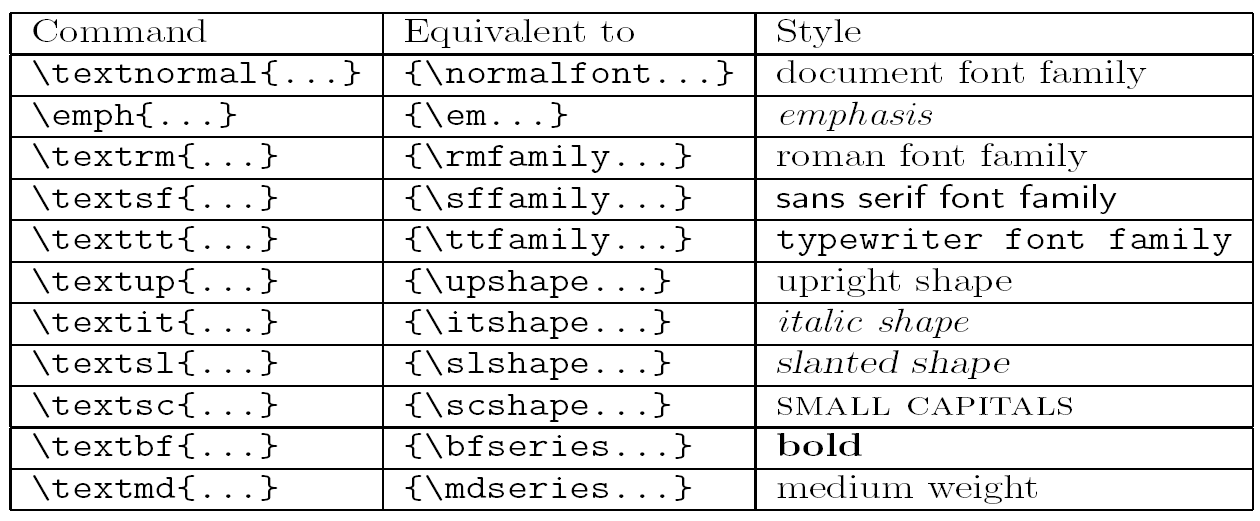
\includegraphics[width=0.7\textwidth]{images/Latex_styles_table.png}
\caption{Available Font styles}
\label{fig:x Available Font styles} \parencite{wiki:003}
\end{figure}



\begin{adjustwidth}{2cm}{2cm}

Examples:

\textsf{This text is written in the sans serif font family}

\textnormal{This text is written in the normal document font family}

\texttt{This text is written in the typewriter family}

We can write some \textbf{bold text}

\textsc{we can write a sentence in small capitals.} 

We can write text with an \emph{emphasis}

We can write text with an \textit{italics}

\end{adjustwidth}

\vspace{0.4cm}

The emphasis command might seem like it is the same thing as italic but it does behave slightly differently. 

\newpage

\section{Font Colours}

In order to use colours in LaTeX we need to ad the \verb|\usepackage{xcolor}| command to the preample in the main.tex file. 

dvipsnames Makes the colour names for the driver dvips available. From this new set of colour names, the example uses: ForestGreen, RubineRed and BurntOrange. See the reference guide for a complete list of possible colours.

There are two very useful commands. 

\verb|\textcolor{color}{text}| and, 

\verb|\colorbox{color}{text}|

\textcolor{blue}{This is an example of blue text}

\colorbox{BurntOrange}{This is an example of a colorbox in BurntOrange}

\textcolor{red}{This whole paragraph is in red text. Curabitur ac augue sit amet enim pretium semper. Ut at finibus ligula. In hac habitasse platea dictumst. Duis porta felis lectus, non sollicitudin turpis ultricies in. Duis tristique justo feugiat elit sollicitudin, at efficitur sapien mollis. Etiam sem nisi, hendrerit vel bibendum non, vehicula vitae nibh.}

\vspace{0.4cm}

\begin{figure}[h]
\centering
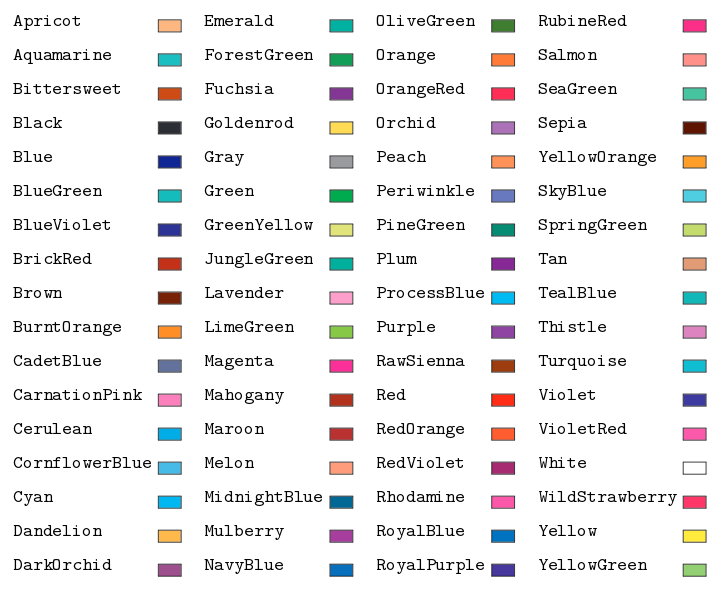
\includegraphics[width=0.7\textwidth]{images/ColoursEx6.png}
\caption{Colour names available with the dvipsnames option}
\label{fig:x Color options} \parencite{overleaf01}
\end{figure}


\newpage

\pagecolor{black}
\color{white}

\section{Page and Font Colours}


It is possible using the \verb|pagecolor{}| \verb|color{}| commands to change to color of a page and font. This page is set to BLACK and the text is set to WHITE.

\vspace{0.4cm}

Lorem ipsum dolor sit amet, consectetur adipiscing elit. Nam rutrum magna ut mi sollicitudin pellentesque. Vivamus sit amet euismod nibh. Sed ornare enim vel tellus faucibus egestas. Donec sit amet diam placerat, interdum sapien sit amet, pulvinar neque. Morbi eget massa ut erat vehicula efficitur. Aenean vitae luctus magna. Nam varius ligula nec nunc egestas ultricies. Quisque vel vehicula mauris. Phasellus venenatis tortor et lorem aliquam luctus.


\textcolor{red}{Lorem ipsum dolor sit amet, consectetur adipiscing elit. Nam rutrum magna ut mi sollicitudin pellentesque. Vivamus sit amet euismod nibh. Sed ornare enim vel tellus faucibus egestas. Donec sit amet diam placerat, interdum sapien sit amet, pulvinar neque. Morbi eget massa ut erat vehicula efficitur. Aenean vitae luctus magna. Nam varius ligula nec nunc egestas ultricies. Quisque vel vehicula mauris. Phasellus venenatis tortor et lorem aliquam luctus.}


Lorem ipsum dolor sit amet, consectetur adipiscing elit. Nam rutrum magna ut mi sollicitudin pellentesque. Vivamus sit amet euismod nibh. Sed ornare enim vel tellus faucibus egestas. Donec sit amet diam placerat, interdum sapien sit amet, pulvinar neque. Morbi eget massa ut erat vehicula efficitur. Aenean vitae luctus magna. Nam varius ligula nec nunc egestas ultricies. Quisque vel vehicula mauris. Phasellus venenatis tortor et lorem aliquam luctus.

\textbf{Lorem ipsum dolor sit amet, consectetur adipiscing elit. Nam rutrum magna ut mi sollicitudin pellentesque. Vivamus sit amet euismod nibh. Sed ornare enim vel tellus faucibus egestas. Donec sit amet diam placerat, interdum sapien sit amet, pulvinar neque. Morbi eget massa ut erat vehicula efficitur. Aenean vitae luctus magna.}


\newpage

\pagecolor{white}

\color{black}

To reset the page and font colors we re-issue the commands \verb|pagecolor{}| and  \verb|color{}| with page colour set back to white and text set to black. 

\vspace{0.4cm}

Lorem ipsum dolor sit amet, consectetur adipiscing elit. Nam rutrum magna ut mi sollicitudin pellentesque. Vivamus sit amet euismod nibh. Sed ornare enim vel tellus faucibus egestas. Donec sit amet diam placerat, interdum sapien sit amet, pulvinar neque. Morbi eget massa ut erat vehicula efficitur. Aenean vitae luctus magna. Nam varius ligula nec nunc egestas ultricies. Quisque vel vehicula mauris. Phasellus venenatis tortor et lorem aliquam luctus.


Lorem ipsum dolor sit amet, consectetur adipiscing elit. Nam rutrum magna ut mi sollicitudin pellentesque. Vivamus sit amet euismod nibh. Sed ornare enim vel tellus faucibus egestas. Donec sit amet diam placerat, interdum sapien sit amet, pulvinar neque. Morbi eget massa ut erat vehicula efficitur. Aenean vitae luctus magna. Nam varius ligula nec nunc egestas ultricies. Quisque vel vehicula mauris. Phasellus venenatis tortor et lorem aliquam luctus.


Lorem ipsum dolor sit amet, consectetur adipiscing elit. Nam rutrum magna ut mi sollicitudin pellentesque. Vivamus sit amet euismod nibh. Sed ornare enim vel tellus faucibus egestas. Donec sit amet diam placerat, interdum sapien sit amet, pulvinar neque. Morbi eget massa ut erat vehicula efficitur. Aenean vitae luctus magna. Nam varius ligula nec nunc egestas ultricies. Quisque vel vehicula mauris. Phasellus venenatis tortor et lorem aliquam luctus.



Lorem ipsum dolor sit amet, consectetur adipiscing elit. Nam rutrum magna ut mi sollicitudin pellentesque. Vivamus sit amet euismod nibh. Sed ornare enim vel tellus faucibus egestas. Donec sit amet diam placerat, interdum sapien sit amet, pulvinar neque. Morbi eget massa ut erat vehicula efficitur. Aenean vitae luctus magna. Nam varius ligula nec nunc egestas ultricies. Quisque vel vehicula mauris. Phasellus venenatis tortor et lorem aliquam luctus.Lorem ipsum dolor sit amet, consectetur adipiscing elit. Nam rutrum magna ut mi sollicitudin pellentesque. Vivamus sit amet euismod nibh. Sed ornare enim vel tellus faucibus egestas. Donec sit amet diam placerat, interdum sapien sit amet, pulvinar neque. Morbi eget massa ut erat vehicula efficitur. Aenean vitae luctus magna. Nam varius ligula nec nunc egestas ultricies. Quisque vel vehicula mauris. Phasellus venenatis tortor et lorem aliquam luctus.


Lorem ipsum dolor sit amet, consectetur adipiscing elit. Nam rutrum magna ut mi sollicitudin pellentesque. Vivamus sit amet euismod nibh. Sed ornare enim vel tellus faucibus egestas. Donec sit amet diam placerat, interdum sapien sit amet, pulvinar neque. Morbi eget massa ut erat vehicula efficitur. Aenean vitae luctus magna. Nam varius ligula nec nunc egestas ultricies. Quisque vel vehicula mauris. Phasellus venenatis tortor et lorem aliquam luctus.


\newpage
